\chapter{The most exciting observable}
\label{ch:nedm-at-psi}

\begin{center}
  \emph{The chief forms of beauty are order and symmetry and definiteness, which the mathematical sciences demonstrate in a special degree.}\\
  Aristotle
\end{center}


\begin{center}
  \emph{Why are we here? Because of CP-symmetry violation.}\\
  prof. Edward Hinds
\end{center}

\section{Symmetries}

% Symmetry is the most fundamental form of beauty.

The essence of the classical physics are the three symmetries: with respect to the spatial translation (homogeneity of space), with respect to rotation (isotropy of space) and with respect to translation in time (homogeneity of time). As Noether showed, they correspond to the conservation laws of momentum, angular momentum and energy, respectively. By saying a symmetry is conserved, we understand that no physical system becomes any different by \emph{only} having been moved in space, rotated, or looked at later.

These are continuous symmetries. No less fundamental is the triad of symmetries with respect to discrete transformations: $P$, parity transformation, mirroring the spatial dimensions; $T$, time reversal, flipping the arrow of the time; and $C$, charge conjugation, flipping \emph{all} charges of particles. One would expect a beautiful universe to work exactly the same in the mirror, or with matter swapped with anti-matter.

Discrete symmetries can be combined. So $CP$ means a symmetry after flipping the charges \emph{and} mirroring the space. The combined $CPT$-symmetry is a mental refuge: any Lorentz invariant local quantum field theory with a Hermitian Hamiltonian. It scares a humble experimental physicist to think of a theory which would not fulfill this.

Yet, in a perfectly symmetric universe after the Big Bang an equal amount of matter and anti-matter would be created and they would perfectly annihilate. There would not be us.
In 1967 Andrei Sakharov
\marginpar{Andrei Sakharov, pacifist and human-rights activist, was awarded the 1975 Nobel Piece Price, called ``a spokesman for the conscience of mankind''.}
has formulated that a necessary condition for that not to happen, for there to be a bit of matter left over, is a violation of the $CP$-symmetry~\cite{0038-5670-34-5-A08}.

Physicist have now long accepted violations of the fundamental symmetries.
The first shock came in 1956 with Chien-Shiung Wu's discovery of $P$ violation in beta decay of cobalt-60~\cite{PhysRev.105.1413}. Shortly thereafter, in 1964, discovery of $CP$ violation in $K^0_L \rightarrow \pi^+ \pi^-$ decay left the physics world stunned again~\cite{PhysRevLett.13.138}. Now both are explained in the scope of the Standard Model of particle physics. In the Model the CP-violation appears in the weak sector as a complex phase in the Cabbibo--Kobayashi--Maskawa matrix---the matrix that mixes the mass- and interaction-eigenstates of quarks. It also appears in the strong sector, as an additional term, parametrised by $\theta_\text{QCD}$. \note{comment more?}

Yet, the $CP$-symmetry in the Standard Model is not enough. The observer matter--anti-matter asymmetry is around $10^{-10}$, while only $10^{-18}$ can be attributed to the Model~\cite{Riotto1999}. Despite the tremendous success of the Standard Model, we know it is not the full picture. We \emph{know} that the CP-symmetry is violated somewhere still, but do not know neither where or how. Naturally, we want to find out. %\cite{Pospelov2005}

Many theories beyond the Standard Model have been proposed that offer to solve this, among others, problem. A very popular idea is to introduce additional particles around the scale of weak interactions (several-hundred GeV), as, for example, supersymmetry does. Those theories typically introduce additional mechanisms of $CP$-violation, which provide an opportunity to test their prediction.



\section{The neutron electric dipole moment}

Excellent probes for these theories are electric dipole moments (EDMs)~\cite{Pospelov2005}. An EDM is a $T$-violating, so assuming $CPT$ conservation, also $CP$-violating observable. In a non-relativistic case of a particle in an electric and magnetic field, with the magnetic and electric moments $mu$ and $d$, the hamiltonian is:
\begin{equation}
  H = - \mu \, \bm{B} \cdot \frac{\bm{S}}{S} - d \, \bm{E} \cdot \frac{\bm{S}}{S} \ .
\end{equation}
For a spin $S = \frac{1}{2}$ particle:
\begin{equation}
  H = - \frac{1}{2} \left( \mu \, \bm{B} + d \, \bm{E} \right ) \cdot \bm{S} \ .
\end{equation}
Vectors, like $\bm{E}$, are $P$-odd, while pseudovectors, $\bm{B}$ and $\bm{S}$, are $P$-even. The hamiltonian as whole is $P$-odd:
\begin{equation}
  H_P = - \frac{1}{2} \left( \mu \, \bm{B} - d \, \bm{E} \right ) \cdot \bm{S} \neq H \ .
\end{equation}
Under the time symmetry the spin is reversed and so is the magnetic field, rendering the hamiltonian $T$-odd:
\marginpar{Magnetic field is produced either by magnetic moments, which flip under $T$ together with spins, or by a movement of charges, which also is reversed under $T$.}
\begin{equation}
  H_T = H_{CP} = + \frac{1}{2} \left( - \mu \, \bm{B} + d \, \bm{E} \right ) \cdot \bm{S} = - \frac{1}{2} \left( \mu \, \bm{B} - d \, \bm{E} \right ) \cdot \bm{S} \neq H \ .
\end{equation}
Note how in both cases setting $d = 0$ restores the symmetry.

EDMs are measured in three main kinds of systems. Beams of cold paramagnetic molecules, like YbF, provide a great sensitivity to the EDM of the electron~\cite{Hudson2011}. Measurements of vapours of diamagnetic atoms, notably $^{199}Hg$~\cite{PhysRevLett.116.161601}, are the most sensitive EDM measurements. Finally, the electric dipole moment of a free neutron, nEDM, which is the topic of this chapter.

Neutron EDM, theories give straightforward predictions~\cite{Ellis1989}. Also, gives handle on theta-QCD.



\section{Measurements of nEDM}

\begin{figure}
  \centering
  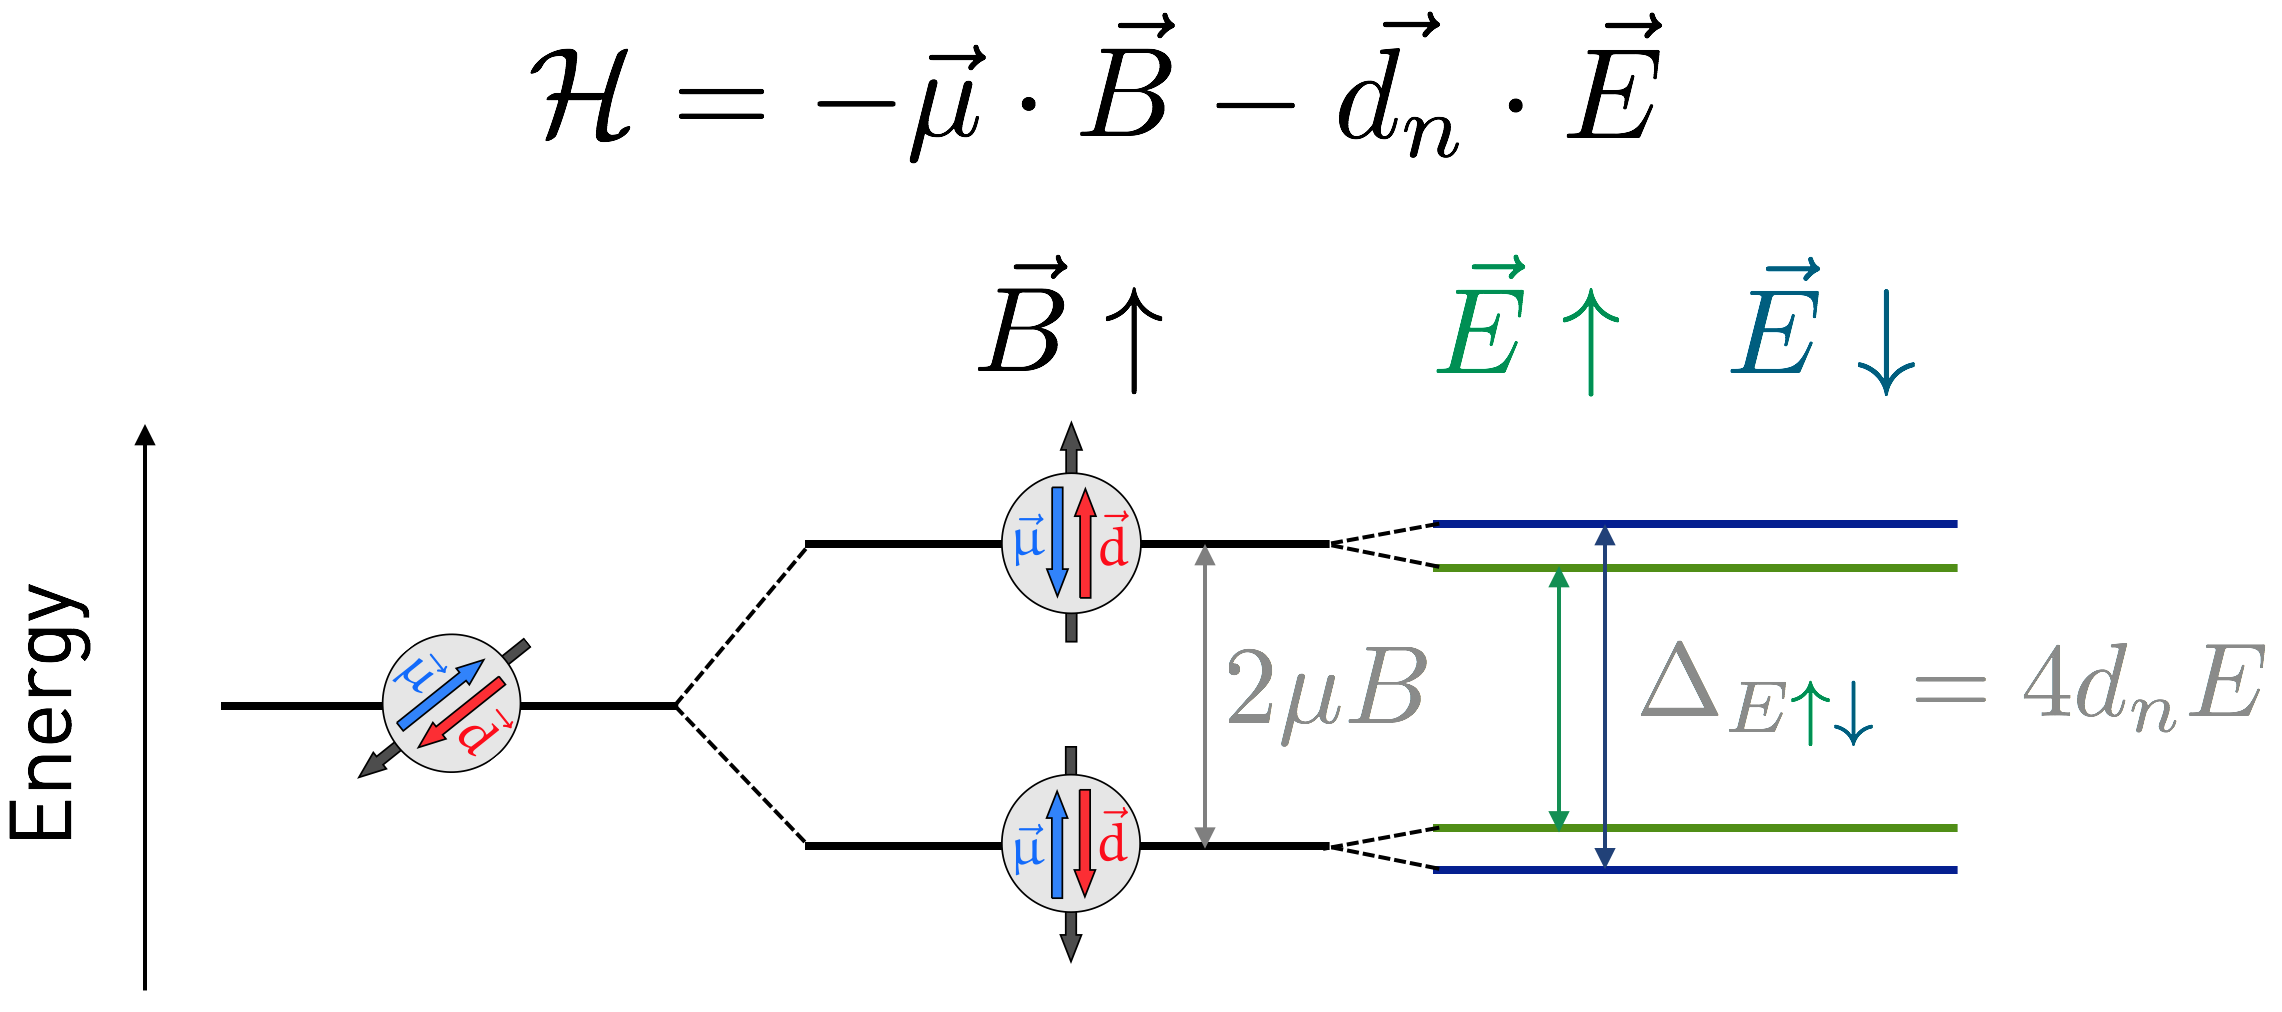
\includegraphics[width=\linewidth]{gfx/nEDMatPSI/measurement_principle.png}
  \caption{\ldots}
  \label{fig:nEDM_measurement_principle}
\end{figure}

Already in 1949, before Wu's discovery of $P$-violation in the weak sector, Purcell and Ramsey performed a measurement to test $P$-violation in the strong sector, using nEDM as the probe~\cite{PhysRev.108.120}. They got a zero-consistent result $d_n = (-0.1 \pm 2.4) \times 10^{-20}\,\si{\elementarycharge\centi\meter}$.

As shown in Fig.\,\ref{fig:nEDM_measurement_principle} a neutron in a magnetic field has two energy states, separated by $2 \mu B$. The apparatus of Purcell and Ramsey could measure this separation, as a frequency, very precisely. Additionally to the magnetic field there was an electric one, either parallel or antiparallel to it. If there had been an nEDM, the energy separation would have increased in one configuration and decreased in the other. The difference between the energy separations measured in the two field configurations is proportional to $d_n$.

\begin{figure}
  \centering
  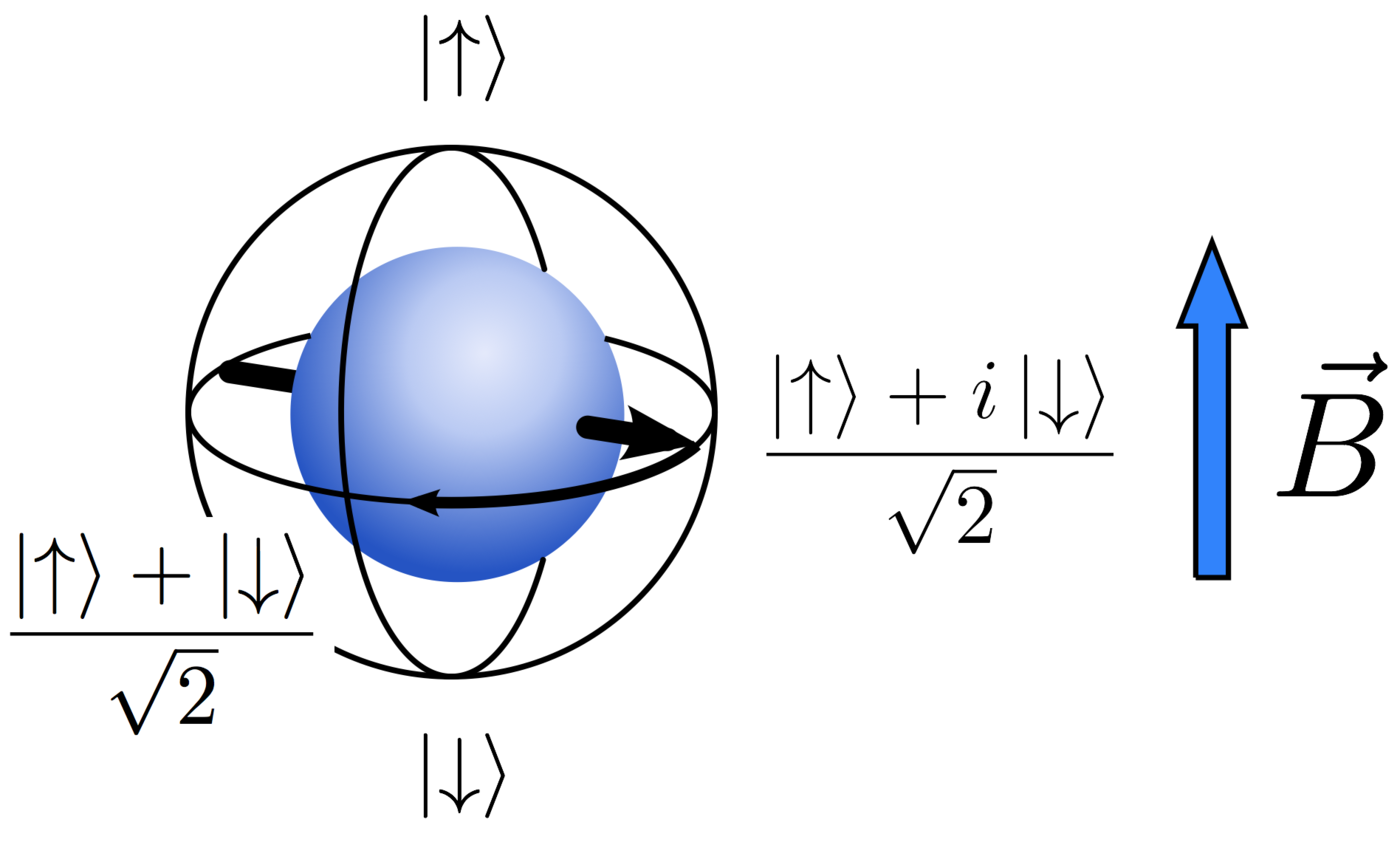
\includegraphics[width=.6\linewidth]{gfx/nEDMatPSI/bloch_sphere.png}
  \caption{\ldots}
  \label{fig:nEDM_bloch_sphere}
\end{figure}

To measure the energy separation between the two spin states they used what is now called the Ramsey method of separated oscillatory fields. To explain it let us first consider a neutron in a magnetic field, as pictured in Fig.\,\ref{fig:nEDM_bloch_sphere}. The neutron's spin is depicted there on the Bloch sphere, where the poles correspond to the spin-up and spin-down states. On the equator lie the states with equal content of spin-up and down, the longitude marking the quantum phase between the two. If the spin lies in the horizontal plane the interaction between the magnetic moment and the magnetic field exerts a torque that sets it into rotational motion, called Larmor precession.

\begin{SCfigure}
  \centering
  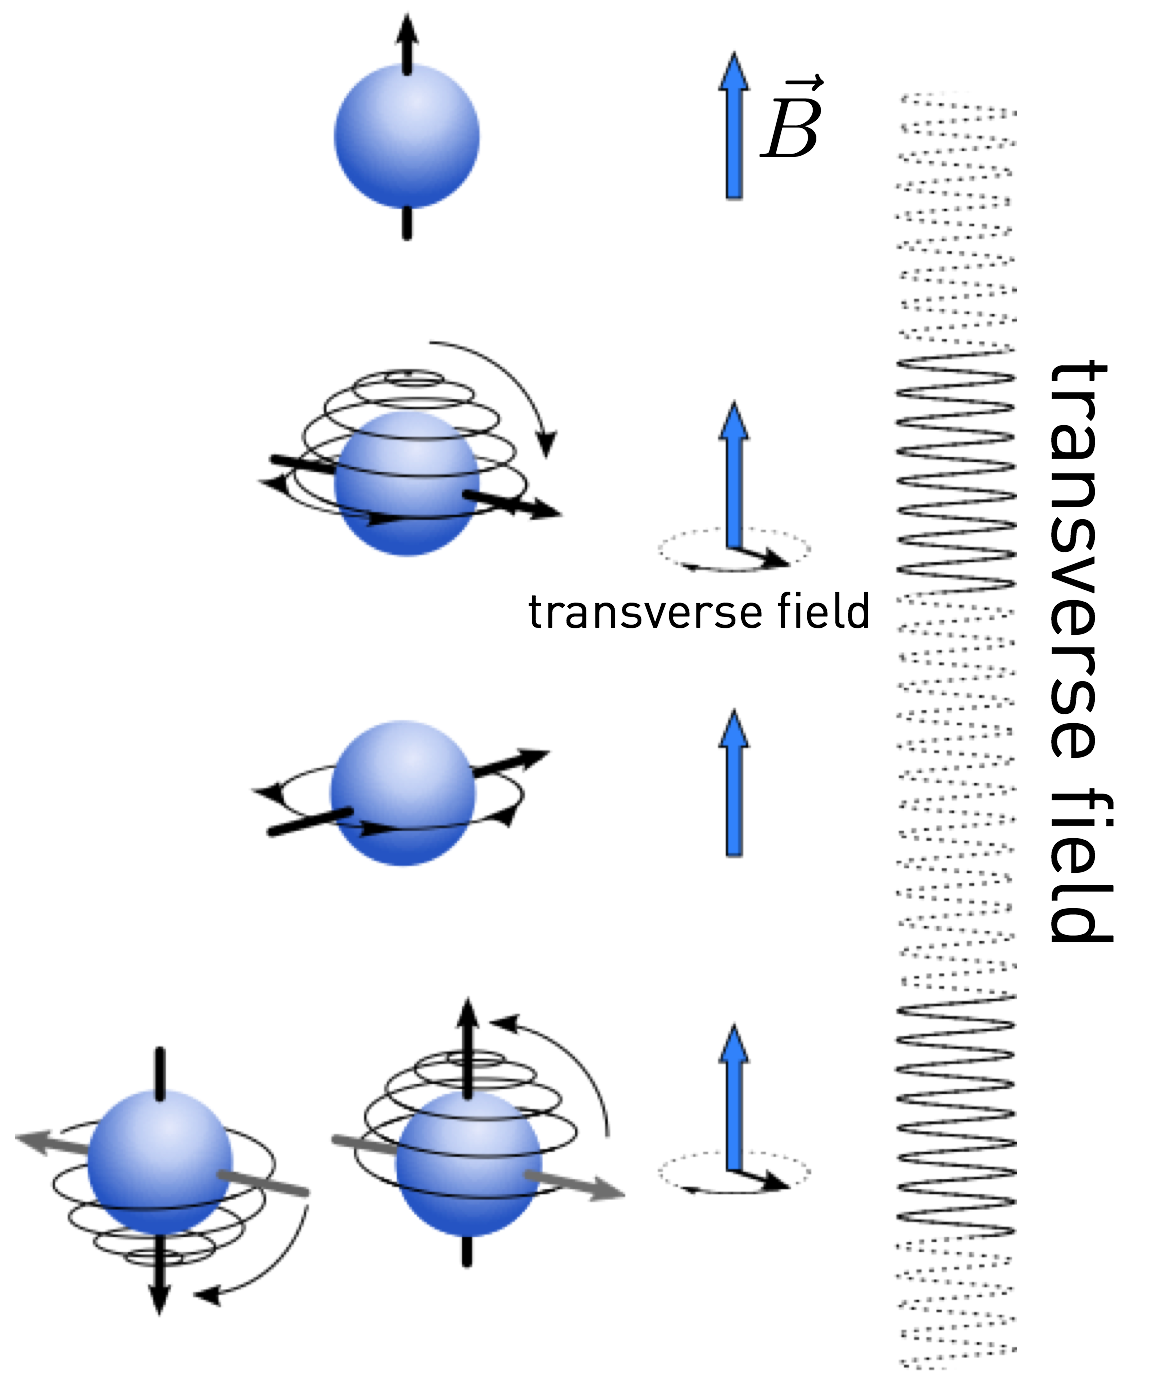
\includegraphics[width=.6\linewidth]{gfx/nEDMatPSI/Ramsey_principle.png}
  \caption{The principle of the Ramsey method, explained with the spin on the Bloch sphere. A polarised spin ensemble is in a magnetic field. A pulse of an oscillating transverse field flips the polarisation into the horizontal plane. The spin is allowed to freely precess in the field. Then, a second pulse of a transverse field is applied, in phase with the first one. The direction of the polarisation's flip depends on the relative phase between the spin and the transverse field.}
  \label{fig:nEDM_Ramsey_principle}
\end{SCfigure}

\begin{figure}
  \centering
  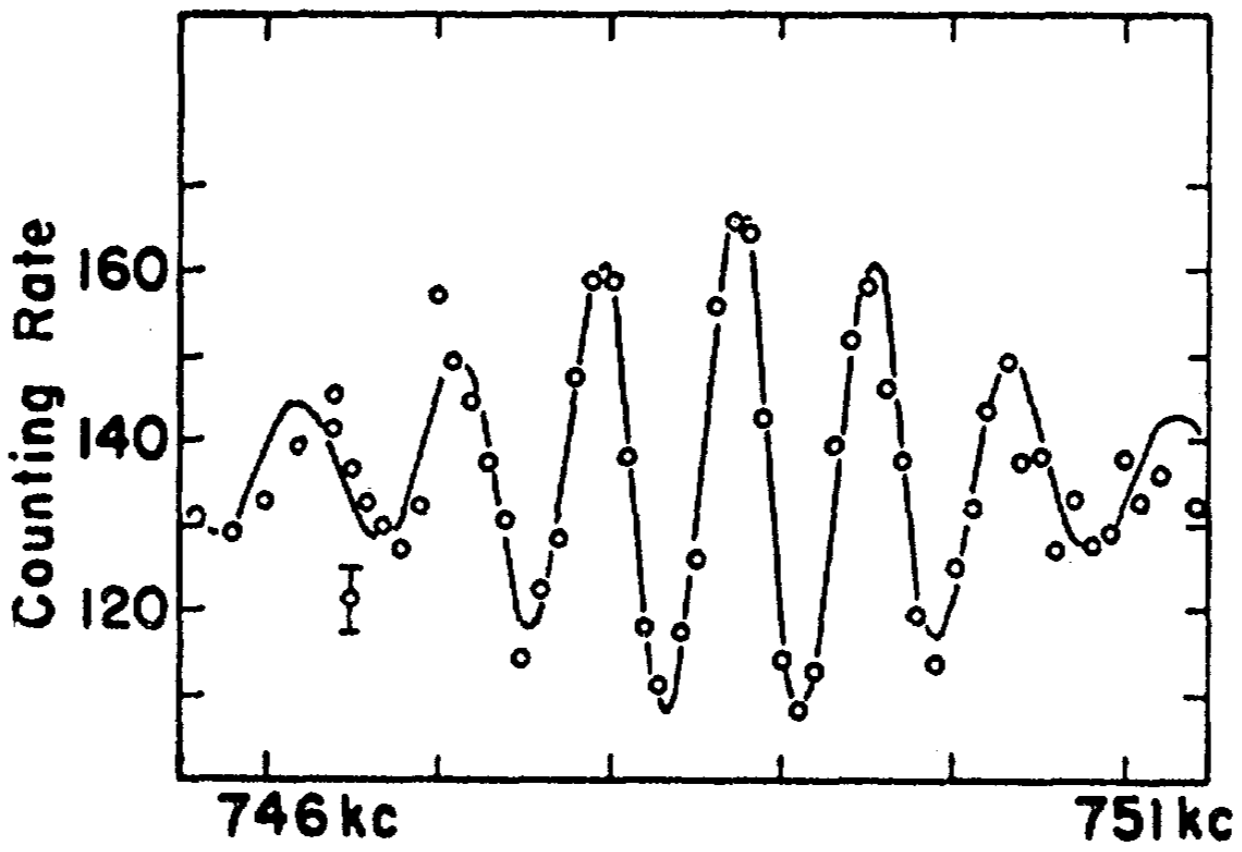
\includegraphics[width=.6\linewidth]{gfx/introduction/Ramsey_original_resonance.png}
  \caption{The original resonance curve measured by Ramsey~\cite{PhysRev.108.120}. The counting rate versus the frequency of the generator powering the spin-flipping coils. The fringes are due the interference between the precessing spins and the transverse field. Their width is the inverse duration of the free precession. The envelope arises, as at a large detuning the spins were not flipped into the horizontal plane anymore.}
  \label{fig:nEDM_Ramsey_original_curve}
\end{figure}

In the experiment the neutron beam passed through a polariser, a region with a magnetic and electric fields, and landed after an analyser on a neutron counter. At the beginning and the end of the region with the fields there were coils producing an oscillating magnetic field in the direction perpendicular to the main field. When a neutron precessing in a magnetic field feels an additional oscillating field, transverse to the main one, and of frequency close to the one of the precession, its spin undergoes nutation---the precession plane moves along the main field. The direction is determined by the relative phase between the spin's precession and the transverse oscillating field. The spin evolution between the two coils is depicted in Fig.\,\ref{fig:nEDM_Ramsey_principle}. The length of the coils was set to flip the neutrons' spins by $\pi/2$, so that after having passed the first coil they were precessing in a plane transverse to the magnetic and electric fields. The direction of the nutation in the second coil, and with it the probability of passing the analyser, depended on the relative phase between the precession and the transverse field. A slight change in the frequency of the generator powering the coils caused a considerable change in the phase that builded up while the neutrons flew precessing between the coils. Scanning the frequency of the generator and monitoring the counting rate gave a resonance curve (Fig.\,\ref{fig:nEDM_Ramsey_original_curve}). The centre of the central fringe is the frequency corresponding to the transition energy between spin-up and spin-down states.

\begin{figure}
  \centering
  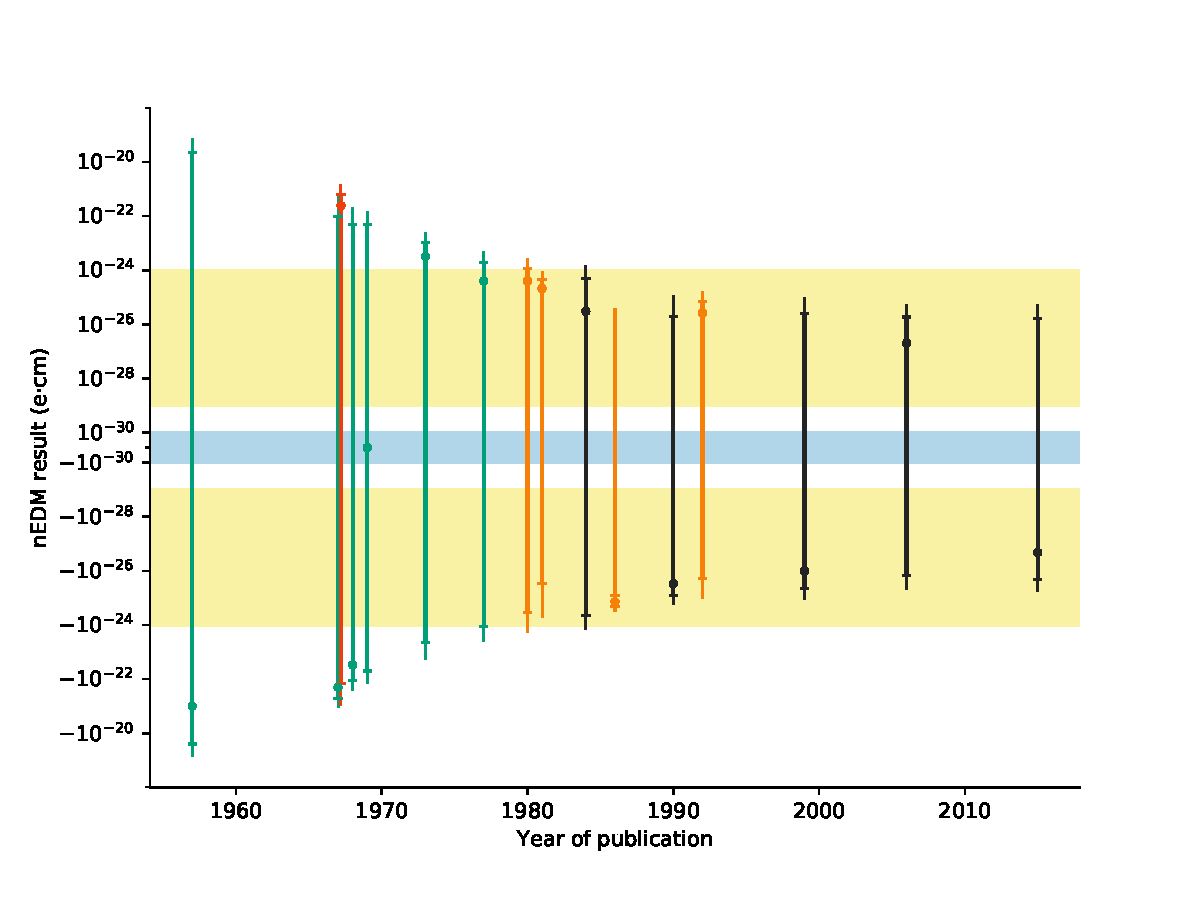
\includegraphics[width=\linewidth]{gfx/introduction/edm_limits.pdf}
  \caption{\ldots \note{Work it over} \note{Make it BOOOM, state-of-the art, with individual points marked, theories marked, make everyone want to steal it!} \note{If I have the time. \cite{PhysRev.108.120,PhysRevLett.19.381,PhysRev.170.1200,PhysRev.179.1285,PhysRevD.7.3147,PhysRevD.15.9,ALTAREV1980269,ALTAREV198113,altarev1986search,ALTAREV1992242,PENDLEBURY1984327,SMITH1990191,PhysRevLett.82.904,PhysRevLett.97.131801}  }}
  \label{fig:nEDM_limits_history}
\end{figure}

The community uses this technique to measure the nEDM until this day. The measurements were done with beam until\ldots. xxxx was the first measurement done with the neurons being stored in a bottle, rather than on a beam. Here a bit on the UCN. The last point is the prediction, the author had the honour of being part of it.
